\documentclass[tikz,border=5pt]{standalone}
\usepackage[dvipsnames]{xcolor}
\usepackage{tikz}
\usetikzlibrary{arrows.meta,calc,fit,positioning,backgrounds,shapes.geometric}

\tikzset{
  component/.style={
    rectangle,
    draw=gray!50!black,
    fill=gray!12,
    rounded corners=2pt,
    minimum width=20mm,
    minimum height=20mm,
    inner sep=0pt
  },
  port/.style={
    rectangle,
    draw=black,
    fill=white,
    minimum width=7.5mm,
    minimum height=7.5mm,
    inner sep=0pt,
    font=\bfseries\small
  },
  eventport/.style={
    draw=blue!70!black,
    fill=blue!8,
    line width=0.6pt,
    minimum width=12.5mm,
    minimum height=7.5mm,
    font=\small\ttfamily,
    inner sep=1pt
  },
  connection/.style={
    thick,
    ->,
    >=Latex
  },
  eventconnection/.style={
    connection,
    dashed,
    blue!75!black
  },
  directfeedthrough/.style={
    ->,
    thick,
    dashed,
    red!75!black
  }
}

\newcommand{\arrowlegend}[1]{%
  \begin{scope}[shift={#1}]
    \draw[->, dashed, thick, red!75!black] (0,0) -- (0.7,0);
    \node[anchor=west, font=\small] at (0.75,0) {direct feedthrough};
    \draw[->, thick, black] (3.8,0) -- (4.5,0);
    \node[anchor=west, font=\small] at (4.55,0) {connection};
    \draw[eventconnection] (6.5,-0) -- (7.2,0);
    \node[anchor=west, font=\small] at (7.25,0) {event connection};
  \end{scope}%
}

\begin{document}
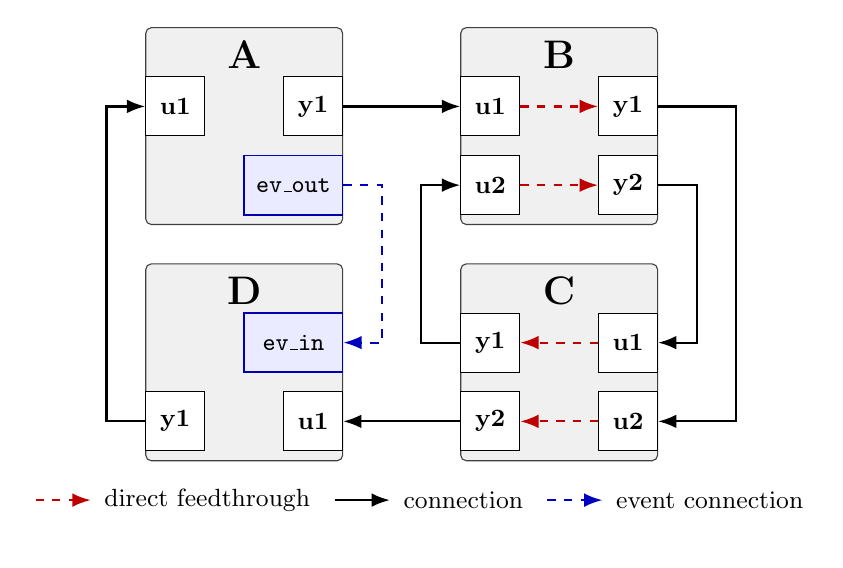
\begin{tikzpicture}[>=Latex]
  % Force identical bounding box across all four panels
  \useasboundingbox (-1.5, -1) rectangle (8.5, 5.5);
  % \draw[help lines, step=0.5] (-1.5,-1) grid (8.5,5.5);

  % Component A
  \begin{scope}[shift={(0,3)}]
    \draw[component] (0,0) rectangle (2.5,2.5);
    \node[anchor=north, font=\Large\bfseries] at (1.25,2.45) {A};
    \node[port] (A-u1) at (0.375,1.5) {u1};
    \node[port] (A-y1) at (2.125,1.5) {y1};
    \node[eventport] (A-y2) at (1.875,0.5) {ev\_out};
  \end{scope}

  % Component B
  \begin{scope}[shift={(4,3)}]
    \draw[component] (0,0) rectangle (2.5,2.5);
    \node[anchor=north, font=\Large\bfseries] at (1.25,2.45) {B};
    \node[port] (B-u1) at (0.375,1.5) {u1};
    \node[port] (B-u2) at (0.375,0.5) {u2};
    \node[port] (B-y1) at (2.125,1.5) {y1};
    \node[port] (B-y2) at (2.125,0.5) {y2};
    \draw[directfeedthrough] (B-u1) -- (B-y1);
    \draw[directfeedthrough] (B-u2) -- (B-y2);
  \end{scope}

  % Component C
  \begin{scope}[shift={(4,0)}]
    \draw[component] (0,0) rectangle (2.5,2.5);
    \node[anchor=north, font=\Large\bfseries] at (1.25,2.45) {C};
    \node[port] (C-y1) at (0.375,1.5) {y1};
    \node[port] (C-y2) at (0.375,0.5) {y2};
    \node[port] (C-u1) at (2.125,1.5) {u1};
    \node[port] (C-u2) at (2.125,0.5) {u2};
    \draw[directfeedthrough] (C-u1) -- (C-y1);
    \draw[directfeedthrough] (C-u2) -- (C-y2);
  \end{scope}

  % Component D
  \begin{scope}[shift={(0,0)}]
    \draw[component] (0,0) rectangle (2.5,2.5);
    \node[anchor=north, font=\Large\bfseries] at (1.25,2.45) {D};
    \node[port] (D-y1) at (0.375,0.5) {y1};
    \node[port] (D-u1) at (2.125,0.5) {u1};
    \node[eventport] (D-listener) at (1.875,1.5) {ev\_in};
  \end{scope}

  \draw[connection] (A-y1) -- (B-u1);
  \draw[connection] (B-y1) --++(1.375,0) --++(0,-4) -- (C-u2);
  \draw[connection] (B-y2) --++(0.375+0.5,0) --++(0,-2) --(C-u1);
  \draw[connection] (C-y1) --++(-0.375-0.5,0) --++(0,2) -- (B-u2);
  \draw[connection] (C-y2) -- (D-u1);
  \draw[connection] (D-y1) --++(-0.375-0.5,0) --++(0,4) -- (A-u1);

  \draw[eventconnection] (A-y2) --++(0.625+0.5,0) --++(0,-2) -- (D-listener);

  \arrowlegend{(-1.4, -0.5)}
\end{tikzpicture}
\end{document}